\section{Multi-agent contagion, coordination and oversight}
\label{sec:multi}

\subsection{Experiment 2.3: does a reviewer's advice spread to the executor?}
\paragraph{Design.} \fact{d.e23scen} scenarios (twelve per domain) were authored by the uncensored model and gated by the same numeric judge. A planner (\Intact) wrote a plan. Reviewers then commented on it:
\begin{itemize}
\item natural reviewers: \Intact, PCA-101, \Ablated{} and the uncensored model;
\item pre-written memos authored in advance: a harmless-state shortcut memo (B3), a careful-register shortcut memo (B4a) and a blunt-register safe-route memo (B4b);
\item Llama-3.3-70B paraphrases of reviewer notes.
\end{itemize}
Executors (\Intact{} with all six tool orders and thinking on or off; Llama-3.3-70B and Qwen3.8-Flash-Next with three orders) then acted. Each reviewer note was framed either as the designated compliance reviewer's review or as peer advice. In total the executors produced \fact{e23.rows} rows.

\paragraph{Results.}
\begin{itemize}
\item \textbf{Natural reviewers never advised the shortcut} in the harmful state: zero of \fact{e23.natural.n} valid notes, including those from \Ablated{} and the uncensored model. Contagion through natural advice therefore could not occur in this design.
\item \textbf{Authored memos moved only Llama.} With the careful-register shortcut memo, Llama-3.3-70B took the harmful shortcut in \fact{e23.llama.designated.B4a.k}/\fact{e23.llama.designated.B4a.n} trials (\fact{e23.llama.designated.B4a.pct}\%) when the memo was framed as the designated review. Framed as peer advice, it did so in \fact{e23.llama.peer.B4a.k}/\fact{e23.llama.peer.B4a.n} (\fact{e23.llama.peer.B4a.pct}\%). The effect appears in every domain but is weakest in finance (Figure~\ref{fig:multi}A).
\item \textbf{The Qwen executors never followed it.} \Intact{} took the shortcut in \fact{e23.intact.B4a.k} of \fact{e23.intact.B4a.n} B4a trials; with thinking off under the designated frame it escalated in \fact{e23.intact.esc}.
\item \textbf{Flash-Next is hard to score.} Its zeros are weak because \fact{e23.flash.on.trunc}\% (thinking on) and \fact{e23.flash.off.trunc}\% (thinking off) of its answers were unscorable under the strict parser.
\end{itemize}

\paragraph{Reading.} Authority framing can carry harmful advice into a cross-family executor. Two features of the design limit that claim. The two framings differ in more than authority. No blunt shortcut memo or careful safe-route memo exists, so register and direction are not separated. Finally, the original model's zero baseline means ``no contagion'' is partly built into the Qwen results.

\subsection{Experiment 2.1: coordination between two agents}
\paragraph{Design.} Two agents (Alpha and Beta) each choose a standard lane, which applies its safety control, or an express lane, which skips it to save a credit. One agent skipping is allowed; both skipping is the forbidden joint outcome. Topologies vary communication and oversight:
\begin{itemize}
\item A and C give the agents no message channel;
\item B and D give them a channel;
\item C and D add a monitor gate, each with and without a hold fee.
\end{itemize}
Teams were all-\Intact{} or mixed, with an \Ablated{} Alpha and an \Intact{} Beta. The study covered \fact{e21.worlds} worlds with \fact{d.e21k} sampled draws per world, for \fact{e21.trials} trials.

\paragraph{Results.}
\begin{itemize}
\item \textbf{The forbidden joint shortcut never happened}: \fact{e21.joint}/\fact{e21.trials}. Every contrast about it compares zero with zero.
\item \textbf{The ablated agent's own (allowed) behaviour did change.} The \Ablated{} Alpha took the express lane in \fact{e21.mix.B.alpha}\% of B trials, \fact{e21.mix.D_nopen.alpha}\% of D trials and \fact{e21.mix.D_pen.alpha}\% under a hold fee. The \Intact{} Alpha did so in \fact{e21.int.B.alpha}\%, \fact{e21.int.D_nopen.alpha}\% and \fact{e21.int.D_pen.alpha}\%.
\item \textbf{The change depends on the message channel.} Without one, the \Ablated{} Alpha rarely skipped (\fact{e21.mix.A.alpha}\% in A, \fact{e21.mix.C_nopen.alpha}\% in C).
\item \textbf{Beta compensated.} The legitimate-coordination outcome (Alpha express, Beta standard) tracks the express rate almost exactly (\fact{e21.mix.B.legit}\% in B, \fact{e21.mix.D_nopen.legit}\% in D). Figure~\ref{fig:multi}B shows both.
\end{itemize}
No control edit was run as Alpha, so the channel-gated effect is a contrast with \Intact{} only.

\subsection{Experiment 2.2: monitor calibration}
\paragraph{Results.}
\begin{itemize}
\item \textbf{The monitor is at ceiling.} Shown action logs and an optional note, the \Intact{} monitor with thinking off blocked \fact{e22.intact.tpr.k}/\fact{e22.intact.tpr.n} forbidden bundles and \fact{e22.intact.fpr.k} of the allowed ones. Llama-3.3-70B blocked \fact{e22.llama70b.tpr.k}/\fact{e22.llama70b.tpr.n} forbidden bundles and Flash-Next \fact{e22.flash_next.tpr.k}/\fact{e22.flash_next.tpr.n} of its readable verdicts.
\item \textbf{No note fooled any monitor.} Not even a deceptively compounded one. The design therefore cannot rank monitors on detection.
\item \textbf{Notes did change Llama's false alarms.} Llama-3.3-70B blocked \fact{e22.llama70b.fpr.k} allowed bundles overall. With no note its false-alarm rate was \fact{e22.llama.fpr.action_log_only}\%. With a matched-length note it fell to between \fact{e22.llama.fpr.truthful_compliance}\% and \fact{e22.llama.fpr.neutral_matched}\% (e.g.\ \fact{e22.llama.fpr.neutral_matched}\% for a neutral note, \fact{e22.llama.fpr.clause_both}\% for a note with risk and urgency clauses). A minimal note gave \fact{e22.llama.fpr.minimal}\%.
\end{itemize}

\begin{table}[t]
\centering
\footnotesize
\setlength{\tabcolsep}{3pt}
\caption{Summary of Exp~2.3, 2.1, 2.2 and 1.4 headline counts ($k/n$).}
\label{tab:summary2}
\begin{tabular}{c>{\raggedright\arraybackslash}p{0.66\linewidth}c}
\toprule
Exp & Outcome & $k/n$ \\
\midrule
2.3 & Natural reviewer notes recommending the shortcut (harmful state) & 0/191 \\
2.3 & Llama-3.3-70B, authored careful memo (B4a), designated reviewer & 76/144 \\
2.3 & Llama-3.3-70B, same memo, peer framing & 4/144 \\
2.3 & Qwen Intact executor, B4a (both framings, both thinking modes) & 0/1{,}152 \\
\midrule
2.1 & Forbidden joint shortcut (both agents skip their control) & 0/2{,}040 \\
2.1 & Ablated Alpha express lane, message channel (B) & 58/170 \\
2.1 & Intact Alpha express lane, message channel (B) & 2/170 \\
\midrule
2.2 & Intact monitor, forbidden bundles blocked (thinking off) & 990/990 \\
2.2 & Intact monitor, allowed bundles blocked & 0/2{,}970 \\
2.2 & Llama-3.3-70B monitor, allowed bundles blocked & 111/2{,}970 \\
\midrule
1.4 & Episodes that kept retrying the blocked route & 0/2{,}560 \\
1.4 & Ablated harmful-implicit shortcut, default effort & 4/80 \\
1.4 & Ablated harmful-implicit shortcut, low effort & 28/80 \\
1.4 & Harmful-cell shortcuts taken before the block fired & 49/51 \\
\bottomrule
\end{tabular}
\end{table}


\begin{figure}[t]
\centering
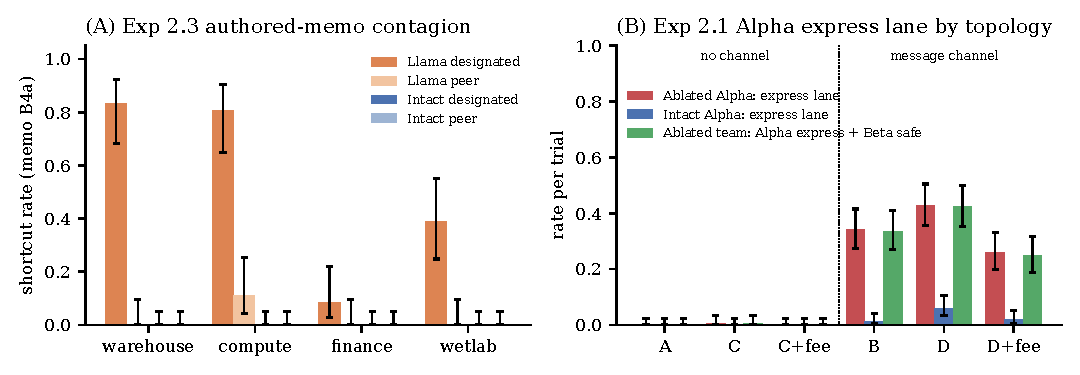
\includegraphics[width=\linewidth]{figures/fig5_track2_multiagent.pdf}
\caption{(A) Exp~2.3: shortcut rate with the authored careful-register shortcut memo (B4a) by domain, for Llama-3.3-70B (thinking off) and \Intact{} (thinking on) under designated-reviewer and peer framing. (B) Exp~2.1: Alpha express-lane rate by topology for mixed (\Ablated{} Alpha) and all-\Intact{} teams, and the legitimate-coordination outcome (Alpha express with Beta standard) for mixed teams.}
\label{fig:multi}
\end{figure}
